\documentclass[xcolor=dvipsnames]{beamer}
\usetheme{Boadilla}

\usepackage{tikz}
\usetikzlibrary{positioning,shapes.misc,arrows,fit,fadings}
\usetikzlibrary{calc}

% Define consistent colors for concepts
\colorlet{CausalColor}{Green}
\colorlet{BiasColor}{Red}
\colorlet{ControlColor}{blue}
\colorlet{PathColor}{Orange}

% Define node styles
\tikzset{
    var/.style={circle, draw, minimum size=0.7cm, inner sep=1pt},
    control/.style={rectangle, draw, fill=ControlColor!20, minimum size=0.7cm, inner sep=1pt},
    highlight/.style={thick, PathColor},
    arrow/.style={->, >=stealth, thick}
    }

    \title{Causal Directed Acyclic Graphs}
    \author{Causal Inference}
    \date{Spring 2026}

    \begin{document}

    \frame{\titlepage}

    %%%%%%%%%%%%%%%%%%%%%%%%%%%%%%%%%%%%%%%%%%%%%%%%%%%%
    \frame{
        \frametitle{Why DAGs?}
        \begin{itemize}
            \item To \textcolor{CausalColor}{visualize} the causal structure of the world.
            \item To identify sources of \textcolor{BiasColor}{bias} in our estimates.
            \item To formally determine which variables we must \textcolor{ControlColor}{condition on}
        \end{itemize}
    }

    %%%%%%%%%%%%%%%%%%%%%%%%%%%%%%%%%%%%%%%%%%%%%%%%%%%%
    \frame{
        \frametitle{Causal Directed Acyclic Graphs (DAGs)}
        \begin{itemize}
            \item A DAG is a visual representation of hypothesized causal relationships.
            \item \textcolor{Red}{\textbf{Directed:}} Each arrow implies a direction of causation (e.g., $X \rightarrow Y$: $X$ causes $Y$).
            \item \textcolor{Green}{\textbf{Acyclic:}} No cycles are allowed (a variable cannot cause itself).
                \vspace{0.2cm}
                \begin{figure}
                    \centering
                    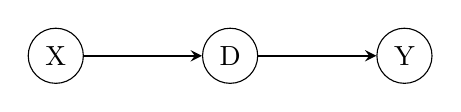
\begin{tikzpicture}[node distance=1.5cm]
                        \node[var] (s1) {X};
                        \node[var, right=of s1] (s2) {D};
                        \node[var, right=of s2] (s3) {Y};
                        \draw[arrow] (s1) edge (s2);
                        \draw[arrow] (s2) edge (s3);
                    \end{tikzpicture}
                    \caption{A simple Causal Chain: $X \rightarrow D \rightarrow Y$}
                \end{figure}
                \vspace{0.2cm}
            \item A \textcolor{PathColor}{\textbf{Path}} is any sequence of edges connecting two variables, regardless of arrow direction.
        \end{itemize}
    }

    %%%%%%%%%%%%%%%%%%%%%%%%%%%%%%%%%%%%%%%%%%%%%%%%%%%%
    \frame{
        \frametitle{The Causal Chain}
        \begin{itemize}
            \item \textbf{Structure:} $D \rightarrow X \rightarrow Y$
            \item Causal association flows freely along this path.
                \vspace{0.2cm}
                \begin{figure}
                    \centering
                    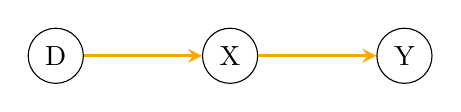
\begin{tikzpicture}[node distance=1.5cm]
                        \node[var] (s1) {D};
                        \node[var, right=of s1] (s2) {X};
                        \node[var, right=of s2] (s3) {Y};
                        \draw[arrow, PathColor, very thick] (s1) edge (s2);
                        \draw[arrow, PathColor, very thick] (s2) edge (s3);
                    \end{tikzpicture}
                \end{figure}
                \vspace{0.2cm}
            \item \textbf{Conditioning on $X$:}
                \begin{itemize}
                    \item $X$ is an \textbf{mediator}
                        \vspace{0.2cm}
                    \item Conditioning on $X$ \textcolor{ControlColor}{blocks} association between $D$ and $Y$.
                \end{itemize}
        \end{itemize}
    }

    %%%%%%%%%%%%%%%%%%%%%%%%%%%%%%%%%%%%%%%%%%%%%%%%%%%%
    \frame{
        \frametitle{The Confounder (The Backdoor Path)}
        \begin{itemize}
            \item \textbf{Structure:} $D \leftarrow X \rightarrow Y$
            \item $X$ is a \textcolor{BiasColor}{\textbf{Confounder}} (or common cause) of $D$ and $Y$.
            \item \textbf{Example:} $D$=Smoking, $Y$=Lung Cancer, $X$=Genetics.
        \end{itemize}
        \begin{figure}
            \centering
            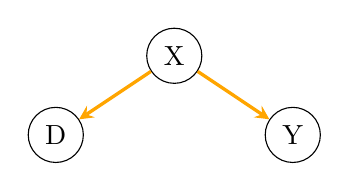
\begin{tikzpicture}[node distance=1.5cm]
                \node[var] (s1) {X};
                \node[var, below left=0.5cm and 1cm of s1] (s2) {D};
                \node[var, below right=0.5cm and 1cm of s1] (s3) {Y};
                \draw[arrow, PathColor, very thick] (s1) edge (s2);
                \draw[arrow, PathColor, very thick] (s1) edge (s3);
            \end{tikzpicture}
        \end{figure}
        \begin{itemize}
            \item \textbf{The Problem:} The path $D \leftarrow X \rightarrow Y$ is a \textcolor{BiasColor}{\textbf{Backdoor Path}}.
            \item Spurious relationship between $D$ and $Y$.
            \item $Pr[Y|D]$ is \textcolor{BiasColor}{biased} because it includes the effect of $X$.
        \end{itemize}
    }

    %%%%%%%%%%%%%%%%%%%%%%%%%%%%%%%%%%%%%%%%%%%%%%%%%%%%
    \frame{
        \frametitle{Conditioning on a Confounder}
        \begin{itemize}
            \item \textcolor{ControlColor}{Condition} on the Confounder $X$ Block the Backdoor Path
                \vspace{0.2cm}
                \begin{figure}
                    \centering
                    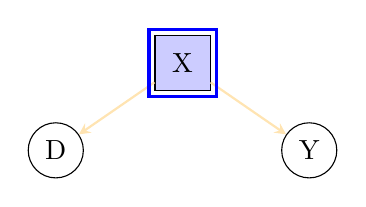
\begin{tikzpicture}[node distance=1.5cm]
                        \node[control] (s1) {X};
                        \node[var, below left=0.5cm and 1cm of s1] (s2) {D};
                        \node[var, below right=0.5cm and 1cm of s1] (s3) {Y};
                        \draw[arrow, PathColor!30] (s1) edge (s2);
                        \draw[arrow, PathColor!30] (s1) edge (s3);
                        \node[fit=(s1), draw=ControlColor, very thick, inner sep=2pt] {};
                    \end{tikzpicture}
                    \caption{Conditioning on $X$ \textcolor{ControlColor}{blocks} the flow.}
                \end{figure}
        \end{itemize}
    }

    %%%%%%%%%%%%%%%%%%%%%%%%%%%%%%%%%%%%%%%%%%%%%%%%%%%%
    \frame{
        \frametitle{The Collider}
        \begin{itemize}
            \item \textbf{Structure:} $D \rightarrow X \leftarrow Y$
            \item \textcolor{ControlColor}{\textbf{Collider}} a node that two arrows point into / shared outcome.
            \item \textbf{Example:} $D$=Student, $Y$=TA, $X$=In This Room.
        \end{itemize}
        \begin{figure}
            \centering
            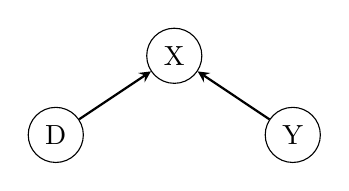
\begin{tikzpicture}[node distance=1.5cm]
                \node[var] (s1) {X};
                \node[var, below left=0.5cm and 1cm of s1] (s2) {D};
                \node[var, below right=0.5cm and 1cm of s1] (s3) {Y};
                \draw[arrow] (s2) edge (s1);
                \draw[arrow] (s3) edge (s1);
            \end{tikzpicture}
        \end{figure}
        \begin{itemize}
            \item The flow of association is \textcolor{CausalColor}{naturally blocked} by a collider.
            \item Marginally, $D$ and $Y$ are independent (e.g., being a student doesn't make you more or less likely to be a TA).
        \end{itemize}
    }

    %%%%%%%%%%%%%%%%%%%%%%%%%%%%%%%%%%%%%%%%%%%%%%%%%%%%
    \frame{
        \frametitle{Conditioning on a Collider}
        \begin{itemize}
                \begin{figure}
                    \centering
                    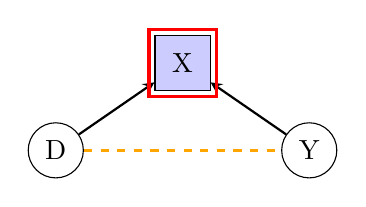
\begin{tikzpicture}[node distance=1.5cm]
                        \node[control] (s1) {X};
                        \node[var, below left=0.5cm and 1cm of s1] (s2) {D};
                        \node[var, below right=0.5cm and 1cm of s1] (s3) {Y};
                        \draw[arrow] (s2) edge (s1);
                        \draw[arrow] (s3) edge (s1);
                        \draw[PathColor, very thick, dashed] (s2) -- (s3); % Show the induced association
                        \node[fit=(s1), draw=BiasColor, very thick, inner sep=2pt] {};
                    \end{tikzpicture}
                    \caption{Conditioning on $X$ \textcolor{BiasColor}{opens} the flow.}
                \end{figure}
            \item Conditioning on the Collider \textcolor{BiasColor}{opens} the path, creating a spurious association between $D$ and $Y$. 
            \item This is called \textit{Collider Bias}.
            \item \textbf{Example:} If we only look at people \emph{in this room} ($X=1$), knowing someone is a student ($D=1$) makes it less likely they are a TA ($Y=0$), because the room is a mix of students and TAs.
        \end{itemize}
    }


    %%%%%%%%%%%%%%%%%%%%%%%%%%%%%%%%%%%%%%%%%%%%%%%%%%%%
    \frame{
        \frametitle{Practice}
        \begin{itemize}
            \item The key is:
                \begin{enumerate}
                    \item \textbf{close all Backdoor Paths} (Confounders) and 
                    \item \textbf{not open any Collider Paths}.
                \end{enumerate}
            \vspace{0.3cm}

            \item Which variables must we condition on?
        \end{itemize}
        \vspace{0.2cm}
        \begin{figure}
            \centering
            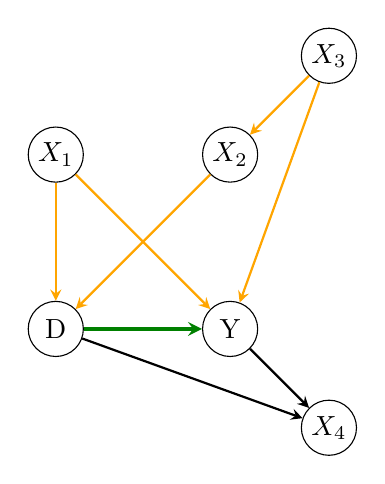
\begin{tikzpicture}[node distance=1.5cm]
                \node[var] (d) {D};
                \node[var, right=of d] (y) {Y};
                \node[var, above=of d] (x1) {$X_1$};
                \node[var, above=of y] (x2) {$X_2$};
                \node[var, above right=0.75cm and 0.75cm of x2] (x3) {$X_3$};
                \node[var, below right=0.75cm and 0.75cm of y] (x4) {$X_4$};

                % Causal Path
                \draw[arrow, CausalColor, very thick] (d) edge (y);

                % Backdoor Path 1: D <- X1 -> Y (Confounder)
                \draw[arrow, PathColor] (x1) edge (d);
                \draw[arrow, PathColor] (x1) edge (y);

                % Backdoor Path 2: D <- X2 <- X3 -> Y (Chain + Confounder)
                \draw[arrow, PathColor] (x3) edge (x2);
                \draw[arrow, PathColor] (x2) edge (d);
                \draw[arrow, PathColor] (x3) edge (y);

                % Path 3: D -> X4 <- Y (Collider)
                \draw[arrow] (d) edge (x4);
                \draw[arrow] (y) edge (x4);
            \end{tikzpicture}
        \end{figure}
        \vspace{0.2cm}
    }

    %%%%%%%%%%%%%%%%%%%%%%%%%%%%%%%%%%%%%%%%%%%%%%%%%%%%
    \frame{
        \frametitle{Summary}
        \begin{itemize}
            \item \textbf{DAGs} are a powerful tool for visualizing and formalizing causal assumptions.
                \vspace{0.2cm}
            \item Backdoor Criterion Revisited: \\

                \vspace{0.2cm}
                A set $S$ is sufficient for adjustment to identify the causal effect of $X$ on $Y$ if:
                \begin{enumerate}
                    \item No element of $S$ is a descendant of $X$ and
                    \item The elements of $S$ block all back-door paths from $X$ to $Y$
                \end{enumerate}
                \vspace{0.2cm}
            \item Condition 1: \textbf{Colliders} must \textbf{not} be \textcolor{BiasColor}{opened} by conditioning.
            \item Condition 2: \textbf{Confounders} (Backdoor Paths) must be \textcolor{ControlColor}{closed} by conditioning.
        \end{itemize}
    }
\end{document}
